%! Author = User
%! Date = 13.09.2023

% Preamble
\documentclass[a4paper,10pt,twocolumn]{article}

% Packages 
\usepackage[utf8]{inputenc}  %man kann Sonderzeiche wie ü,ö usw direkt eingeben
\usepackage{amsmath}           %macht
\usepackage{amsfonts}          %       Mathe
\usepackage{amssymb}           %              mächtiger
\usepackage{graphicx}          %erlaubt Graphiken einzubinden (.eps für dvi und ps sowie .jpg für pdf)
\usepackage[T1]{fontenc}       %Zeichenbelegung der verwendeten Schrift
\usepackage{ae}                %macht schöneres ß
\usepackage{typearea}
\usepackage{amstex}
\usepackage{siunitx}
\usepackage{hyperref}	         %ermöglicht änderung des Seitenspiegels
\usepackage{subcaption}


\usepackage{amsmath}
\usepackage{tikz}
\usepackage{pgfplots}

\newcommand{\alphaNoError}{(4.047 \pm 0.036)}
\newcommand{\betaNoError}{(-4.73 \pm 0.29) \cdot 10^{-3}}
\newcommand{\halfTimeNoError}{(146.5 \pm 9.1)\ s}
\newcommand{\alphaGauss}{(4.04 \pm 0.10)}
\newcommand{\betaGauss}{(-4.62 \pm 0.95) \cdot 10^{-3}}
\newcommand{\halfTimeGauss}{(150 \pm 31)\ s}
\newcommand{\alphaPoisson}{(4.05 \pm 0.10)}
\newcommand{\betaPoisson}{(-4.75 \pm 0.95) \cdot 10^{-3}}
\newcommand{\halfTimePoisson}{(146 \pm 29)\ s}
\newcommand{\symN}{\delta N}



\pagestyle{scrheadings}        %sagt Koma-Skript, dass selbstdefiniers Kopfzeilen verwendet werden
\typearea{16}                  %stellt Seitenspiegel ein
\columnsep25pt								 %definiert Breite zwischen den zwei Spalten von \twocolumns

\renewcommand{\pnumfont}{%     %ändert die Schriftart der Seitennummerierung
    \normalfont\rmfamily\slshape}  %ändert die Schriftart der Seitennummerierung 



\begin{document}
    \twocolumn[{\csname @twocolumnfalse\endcsname                %erlaubt "Abstrakt" über beide Spalten
    \titlehead{                                                  %Kopfzeile
        \begin{tabular*}{\textwidth}[]{@{\extracolsep{\fill}}lr}   %Kopfzeile
            Tutor: Johanna Klos & \today\\                          %Kopfzeile - Betreuer
        \end{tabular*}                                             %Kopfzeile
    }
    \title{Magnetic hysteresis curves and characteristic magnetic properties of two industrial Fe-Ni-Alloys and 
    construction steel}  %Titel der Versuchs
    \author{Salahudin Smailagić und Thomas Karb}                     %Namen der Studenten
    \date{}                                                         %benötigt um automatisches Datum auszuschalten
    \maketitle                                                      %erzeugt Titelseite
    \vspace{-5ex}                                                   %verringert Abstand zur Überschrift
    \begin{abstract}                                                %Beginn des Abstracts
        We present a method to study magnetic properties of ferromagnetic materials.
        For three exemplary materials their distictive hysterises curves are recorded.
        We show how to identify the characteristic attributes: coercivity, remenance-field and the
        energy-loss for one loop.
        Their theoretical origin and their affect on the usage of the material are explained.
        With our setup we did not reach the saturation field, but we demonstrate how you can verify from the curve
        weather you have reached the saturation point.
        Lastly a paramagnetic material is examined as comparison.
        It's susceptibility was determined.
        As the theory suggests, its permeability is much lower compared to the ferromagnetic cores.
        \\
        Measuerement made: 21. September 2023\\       %Datum ändern!
        Submitted: 6. October 2023                %Datum ändern!
        \\
        \\
    \end{abstract}
    }] 
    \section{Introduction}
    
    For industrial applications such as transformers, electric motors, etc. it is important to know how ferromagnetic
    materials behave and conduct magnetic fields.
    We want to study these effects and analyse them.
    With a simple setup of two coils, we can measure the conducted magnetic field of the ferromagnetic cores.
    Since the magnetization of a ferromagnetic material also depends on the magnetization-history, we get distinctive hysteresis curves.
    This time dependence is important for explaining permanent magnetism and how much energy is lost when you flip the
    polarisation of the material.
    As it occurs for example in transformers.
    We show how you can extract from the captured data these important properties.
    For three exemplary materials this method is demonstrated.
    The method can then be used in an industrial context for analysing utilized ferromagnetic materials.
    
    \section{Theory}
    \label{sec:Theory}
    
    The magnetic properties of a material are caused by the spins of the electrons.
    In a ferromagnetic material the individual spins of the electrons do not cancel each other out, so every atom has a
    resulting spin.
    But every spin creates a magnetic dipole moment.
    Meaning every atom carries a magnetic dipole moment.
    In a ferromagnetic material the spin of neighboring atoms couple,
    creating domains where the atomic spins are aligned. 
    Those domains, also called Weiss domains, are separated by small boundaries, only a few atoms wide\cite{feymanLecturesWeisDomains}.
    In the 'unmagnetized' state the magnetic dipole moments of each Weiss domain, cancel each other out, resulting in
    a magnetic field of zero.
    If you now apply an external magnetic field the boundaries of the Weiss domains move, so the magnetic moments of the
    domains align with the direction of the applied H-field.
    So the H-Field gets amplified by a large amount.
    
    But the Weiss domains alone, would not explain permanent magnets and hysteresis. 
    In a perfect isotropic cristal, if you would first polarize the cristal and then unpolarize it, 
    the Weiss domains would first align with the H-field and then simply go back to their initial state of lowest energy.
    Thus there would be no remanence field left, as seen in ferromagnetic materials.
    
    A real ferromagnetic material on the other hand is anisotropic.
    It has defects on the cristal lattice.
    After removing the external H-Field, the boundary walls get pinned on those defects.
    So the Weiss domains can not go back in their initial configuration, thus the material stays magnetized.
    This effect results in the hysteresis curve.
    
    You can release the walls of their pinned state by heating the material, by causing vibrations through e.g.: hammering,  
    or by applying an oscillating external B-field as shown in section ~\ref{subsec:steel}.
    
    The hysteresis curve is characterized by a multitude of properties:
    If you apply the H-field the weiss domains will align.
    Thus amplifying the B-field. 
    By increasing the H-field even more, all dipole moments will be aligned and there is no amplification anymore.
    This saturation state is characterized by the threshold $B_{sat}$.
    After wards the B-field only increases with the vacuum permeability $\mu_0$.
    Now after removing the external H-field, the remaining B-field is called remanence $B_{R}$.
    The coercivity $H_C$ is the magnetic force (H-field) the material can withstand, without being demagnetized.
    
    Moving the weiss domains, costs energy.
    This energy loss, when cycling the hysteresis curve, can be calculated with the material density $\rho$:
    
    \begin{align}
        \label{eq:EnergyLoss}
        \xi = \frac{E}{m} = \frac{1}{\rho} \oint{B dH}
    \end{align}
    
    This is the area under the hysteresis curve.
    
    \section{Experimental setup}
    
    \begin{figure}[htbp]
        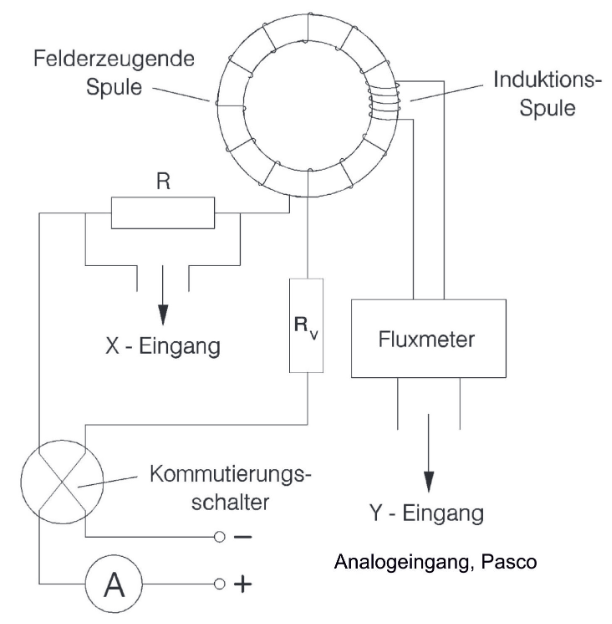
\includegraphics[width=0.9\linewidth]{ExperimentalSetup}
        \caption{Setup for capturing hysteresis curves.
        Channel X of the digital interface measures the current in the field-creating-coil $N_1$.
        The ring core conducts the H-field.
        The resulting B-field is measured by the induction-coil $N_2$.
        The flux meter integrates analogously the voltage of the induction coil and its output is captured by
        channel Y.
        This enables to calculate the B-field at the induction-coil.}
        \label{fig:ExperimentalSetup}
    \end{figure}
    
    We have four ring cores of different materials.
    To capture their magnetic properties we use the experimental setup shown in figure ~\ref{fig:ExperimentalSetup}. 
    The external magnetic field is created by the first coil $N_1$.
    We measure the current via the voltage drop $U_{in}$ at the first resistor.
    Captured by the digital interface at Channel X.
    For small currents we use $R = (66.7 \pm 1.4) \Omega$, else we use $R = 0.20 \Omega$.
    The field created by the first coil can then be calculated with:
    \begin{align}
        \label{eq:CalculateHField}
        H = \frac{N_1}{\frac{\pi}{2}(d_i + d_o)R}U_{in}
    \end{align}
    Where $d_i$ and $d_o$ are the inner and outer diameter of the ring core and $N_1$ is the winding number of the
    field-creating-coil.
    
    The ring core conducts the field and induces a current in the second coil $N_2$.
    To assess the conducted B-field, we use a flux-meter, which integrates analogously, the flux change of the second coil.
    It's output is then captured by channel Y of the digital interface.
    
    The induced current depends on the effective area penetrated by the conducted field.
    \begin{align}
        \label{eq:EffectiveAreaOfInductionCoil}
        A_{eff} = \frac{1}{2} (d_o - d_i) h f
    \end{align}
    Here $h$ is the height of the second coil and $d_o$ and $d_i$ the outer and inner diameter.
    Furthermore $f$ is the effective percentage by which the ring core is filled with the ferromagnetic material.
    This has to be account for since the second and third ring core consist of $0.1 mm$ thin Fe-Ni-bands, which are coated by a oxid layer.
    The effective fill percentage of these cores is $f = 90\%$.
    
    Via Ampere's law you can calculate the induced current by the B-field.
    Therefor with the integrated current measured at channel Y: $U_{out}$, you can infer the conducted field:
    \begin{align}
        \label{eq:CalculateBField} 
        B = \frac{\gamma_f}{N_2 A_{eff}} U_{F}
    \end{align}
    Where $\gamma_f$ is the integration factor of the flux meter.
    
    Since the flux meter integrates analogously, there is an undetermined integration constants shifting the output
    voltage $U_{out}$.
    This shift is corrected by centering the data afterwards.
    Furthermore the capacitor of the flux meter discharges naturally over time.
    This results in a constant drift of the output voltage,
    especially for small currents (compare section~\ref{subsec:fluxDrift}).
    The following data is adjusted for both those effects.
    
    \section{Hysteresis curves}
    \subsection{Steel ST37K}
    \label{subsec:steel}
    
    \figExCoercivityRemanenceSteel{Hysteresis curve for steel ST37K\@.
    Via linear regression the coercivity $H_C = \CoercivitySteel$ and remanence $B_R = \RemanenceSteel$ was accessed.
    Furthermore with numerical integration the energy loss after equation~\eqref{eq:EnergyLoss} is $\xi = \HysteresisLossSteel$.
    The saturation point was not reached.}
    
    We examined a ring core made of common construction steel ST37K\@.
    The captured hysteresis curve can be seen in figure~\ref{fig:ExCoercivityRemanenceSteel}.
    To get the coercivity and remanence we apply linear regression around the H- and B-axis respectively.
    Since the the curve is in proximity of the intersection linear.
    \begin{align*}
        H_C &= \CoercivitySteel \\
        B_R &= \RemanenceSteel
    \end{align*}
    The error was inferred by the statistical scattering of the data points around the linear regression.
    Please be aware that this approach only reflects statistical errors.
    In our measurements we have a large amount of systematical errors, due to the fact that magnetic hysteresis is
    highly dependent on the geometry of the used ring cores. 
    Moreover depending on the manufacturing process, the grain size varies, which greatly affects the permeability of
    the material.
    To make our results reproducible, a far greater control over these factors would be required.
    Because this paper is more concerned with qualitative results, all quantitative results only really apply for the
    local setup used by us.
    
    The energy loss was calculated by numerical integrating the curve and applying equation~\eqref{eq:EnergyLoss}:
    \begin{align*}
        \xi = \HysteresisLossSteel
    \end{align*}
    Similarly the error was determined by the statistical scattering of the data points.
    
    To determine the area under the curve we also tried the alternative approach of cutting out paper-curves and
    weighing the cutout.
    This turned out to be inaccurate.
    See appendix~\ref{subsec:ManualIntegration} for the results.
    
    \subsubsection*{Irreversibility of hysteresis}
    
    \figExIrreversibilitySteel{Hysteresis curve for ST37K.
    By briefly changing direction of the applyied H-field a hysteresis-branch is formed.
    This shows the time dependence of ferromagnetical materials. 
    It can be explained via Weiss domains (c.f. section~\ref{sec:Theory})}
    
    As stated in section~\ref{sec:Theory}, the hysteresis curve depends on the magnetization history
    of the material. 
    This effect can be revealed by briefly flipping the direction of the external H-field.
    Compare figure~\ref{fig:ExIrreversibilitySteel} where after changing the field direction a branch in the curve
    is formed.
    The magnetization does not return to its previous state, instead it is weaker.
    
    This is due to the fact, that moving the boundaries over the lattice defects costs energy $E_{def}$.
    As you can see in figure~\ref{fig:ExIrreversibilitySteel} if we start in a polarized state
    and now remove the H-field, the magnetic moments scatter, to reach an energetic more favorable state.
    We get energy $E_{moments}$.
    So the energy change is:
    \begin{align*}
        \Delta E &= E_{moments} - E_{def}
    \end{align*}
    If we now increase the H-field and polarize the material again, we have to again put in this energy $E_{moments}$.
    But it still costs energy to move the boundaries between the weiss domains over defects $E_{def}$.
    So the energy change is:
    \begin{align*}
        \Delta E &= - E_{moments} - E_{def}
    \end{align*}
    But this means we have overall lost energy, thus the polarisation has to be weaker.
    
    This fact holds also true if we traverse the whole hysteresis loop.
    We have determined this exact energetic loss in the previous section to be:
    \begin{align*}
        \xi = \HysteresisLossSteel
    \end{align*}
    
    \subsubsection*{Demagnetization}
    
    \figExDemagnetizationSteel{Hysteresis curve for steel ST37K.
    The steel was demagnetized by continously flipping and decreasing the applied H-field.
    Because of energy losses, the magnetization gets weaker every time you reverse the H-field.
    In the inlet can be seen, we did not exactly reach a state of complete demagnitization.
    This is due to the constraint, that we did control the H-field manually.}
    
    As shown in the previous section, after you reverse the rate of change of the external field, the magnetisation
    is weaker as in the previous state.
    You can use this fact to demagnetize the material.
    This was achieved by periodically flipping the H-field and decreasing its strength each step,
    The magnetic moments of the weiss domains get more and more disordered, until no remanence-field is left.
    The lowest energetic state is reached.
    
    As you can see in figure~\ref{fig:ExDemagnetizationSteel} we did not reach the state of demagnetization perfectly.
    This is due the fact, that we controlled the H-field manually.
    
    \subsection{PERMENORM 5000 H2 Fe-Ni-Aloy}
    
    \figExSaturationFeNiHTwo{Captured hysteresis curve for 0.1mm thick Fe-Ni 'PERMENOR 5000 H2' strips.
    To test if we have reached the saturation, a line was fitted at the end of the curve.
    The determined permeablity is $\mu = \SaturationPermeabilityFeNiHTwo \mu_0$.
    This means we have not reached the saturation point, where the permability should be $\mu = \mu_0$.}
    
    The second core, which we examined, consisted of the industrial Fe-Ni-Alloy 'PERMENORM 5000 H2'.
    It is constructed out of 0.1 mm thin metal bands.
    The thickness of the metal strips greatly influences the magnetic properties of the material~\cite{feniDatasheet}.
    For the measurement we used the former setup but with the additional resistor $R = (66.7 \pm 1.4) \Omega$,
    to have a higher resolution, since we had a maximum current of $I = 100mA$.
    
    By applying linear regression, we determine the coercivity and remanence field.
    Furthermore via numerical integration we calculated the energy loss.
    \begin{align*}
        H_C &= \CoercivityFeNiHTwo \\
        B_R &= \RemanenceFeNiHTwo \\
        \xi &= \HysteresisLossFeNiHTwo
    \end{align*}
    
    As mentioned these values have a high degree of systematical uncertainty.
    We can compare them with the datasheet of the manufacturer~\cite{feniDatasheet}.
    The coercivity for 0.35mm thick 'PERMENORM 5000 H2' strips is:
    \begin{align*}
        H_C &= 3 \ A/m
    \end{align*}
    Our results are in the same order but do not agree.
    This is due to the fact that there is no datasheet for 0.1mm thick strips publicly available.
    But the thickness as a high impact.
    Further the values of the datasheet have a large uncertainty themself.
    
    As mentioned in section~\ref{sec:Theory} there is a point where the applied H-field is great enough,
    so all magnetic moments are aligned.
    At this saturation point there is no amplification of the magnetic field.
    The slope of the hysteresis curve is $\mu_0$.
    
    To test, weather we have reached the saturation point, we fit a line at the end of the hysteresis
    curve as shown in figure~\ref{fig:ExSaturationFe-Ni H2}.
    The field and the permeability are:
    \begin{align*}
        B_S &= \SaturationFeNiHTwo \\
        \mu &= \SaturationPermeabilityFeNiHTwo \ \mu_0
    \end{align*}
    Obviously we have not reached the saturation point.
    The datasheet confirms this.
    It states, the saturation magnetization at $H = 40 \ kA/m$ to be:
    \begin{align*}
        B_S &= 1.60 \ T
    \end{align*}
    In our measurement we did not reach such a strong H-field.
    The coils did not withstand such high currents.
    A more robust setup would be required.
    
    If we compare this Fe-Ni-Alloy to the previous core out of steel ST37K, we see the alloy as a much lower coercivity and subsequent energy
    loss.
    This makes it ideal for applications in current transformers and magnetic shielding~\cite{feniDatasheet}.
    
    \subsection{PERMENORM 5000 Z Fe-Ni-Aloy}
    
    \figExFeNiZ{Hysteresis curve for the Fe-Ni-Alloy 'PERMENORM 5000 Z'.
    It also consists of 0.1mm thin strips.
    The maximum permeablity is high, while the coercivity is still low $H_C = \CoercivityFeNiZ $.
    The material can also be used for transformer cores, magnetic shielding and current and positioning 
    sensors~\cite{feniDatasheet}.
    }
    
    The third core consisted of the Fe-Ni-Alloy 'PERMENORM 5000 Z'.
    It is also constructed out of 0.1mm thin Fe-Ni-strips.
    Analogously to the coercivity, remanence and energy loss was calculated:
    \begin{align*}
        H_C &= \CoercivityFeNiZ \\
        B_R &= \RemanenceFeNiZ \\
        \xi &= \HysteresisLossFeNiZ
    \end{align*}
    
    Also to test weather we have reached the saturation point, we determined the permeability at the end of the curve:
    \begin{align*}
        B_S &= \SaturationFeNiZ \\
        \mu &= \SaturationPermeabilityFeNiZ \ \mu_0
    \end{align*}
    Obviously the saturation point was also not reached.
    There is no datasheet publicly available to verify these results.
    
    Since the maximum permeability is quite high as seen in figure~\ref{fig:ExFe-Ni Z} and the coercivity is still
    low, the material can also be used in transformers, magnetic shields and current and positioning sensors~\cite{feniDatasheet}.
    
    \subsection{Wood as reference}
    
    \figMessreiheKernFourOneEightTwoRWood{Paramagnetic amplification by a ring core consisting of wood.
    Via regression the susceptibility was calculated: $\chi &= \WoodMagneticSusceptibility$.
    The susceptibility is very high, which makes the material superparamagnetic.
    Probably the core does not consist of wood after all.
    We can not verify this, because we did not build the core.}
    
    To compare our results, we examined a core made of wood as an example for a paramagnetic material.
    
    Paramagnetism is caused by magnetic moments of unpaired spins\cite{gerth}.
    Similarly to ferromagnetism these magnetic moments do align, when an external H-field is applied,
    and thus amplifying it.
    But in contrast to ferromagnetism, no weiss domains are formed, meaning the polarisation does not depend
    on the history.
    Furthermore the amplification by paramagnets is weak.
    The susceptibility is generally in the order of:
    \begin{align*}
        \chi  &\sim 10^{-5}
    \end{align*}
    
    As you can see in figure~\ref{fig:Messreihe_Kern4_18_2_RWood} in our measurements, no hysteresis curve was formed.
    This shows the examined material is paramagnetic.
    The susceptibility was determined by fitting a line in the data points.
    \begin{align*}
        \chi &= \frac{\mu}{\mu_0} - 1 = \WoodMagneticSusceptibility
    \end{align*}
    
    The measured susceptibility is much higher as would be expected from a paramagnetic material.
    In fact the susceptibility is great enough, that the material can be considered superparamagnetic.
    Probably the core did not solely consist of wood.
    There has to be another material part of the core.
    Maybe it is a ferromagnet above the curie temperature, since they exhibit superparamagnetic behaviour.
    We can not verify these theories, because we did not build the cores.
    A closer inspection would be required.
    
    \section{Summary}
    
    We wanted to examine the characteristic hysteresis curve for ferromagnetic materials.
    For this we used a setup of two coils.
    The first on creates the H-field.
    This field is then conducted by the ferromagnetic core, and induces a current in the second coil.
    Via analog integration we can determine the conducted B-field.
    
    For three ferromagnetic materials we tested this setup.
    For steel ST37K we captured the hysteresis curve and via linear regression we calculated the coercivity
    $H_C = \CoercivitySteel$ and the remanence field $B_R = \RemanenceSteel$.
    Furthermore with numerical integration we can calculate the energy loss of traversing on hysteresis loop:
    $\xi = \HysteresisLossSteel$.
    The irreversibility of hysteresis was shown by briefly flipping the direction of the H-field.
    This was then applied to demagnetize the steel core, by continuously flipping the direction till now remanence-field
    was left.
    
    We repeated this process for the industrial Fe-Ni alloy 'PERMENORM 5000 H2'.
    It is a soft magnetic material.
    It coercivity was measured to be $H_C = \CoercivityFeNiHTwo$, the remanence $B_R = \RemanenceFeNiHTwo$
    and the energy loss $\xi = \HysteresisLossFeNiHTwo$.
    We tested weather we have reached the saturation point by applying a linear fit at the end of the curve.
    The measured slope was $\mu = \SaturationPermeabilityFeNiHTwo \ \mu_0$, which means we did not reach saturation.
    Far greater H-Fields would be required.
    
    For the magnetically harder alloy 'PERMENORM 5000 Z' the characteristic properties were:
    $H_C = \CoercivityFeNiZ$, $B_R = \RemanenceFeNiZ$ and $\xi = \HysteresisLossFeNiZ$.
    Here we also did not reach the saturation point.
    
    Lastly a paramagnetic core was examined.
    It's susceptibility was measured as $\chi = \WoodMagneticSusceptibility$.
    This would make the core superparamagnetic.
    
    Please note all stated values above only really apply for our local setups. 
    Magnetic hysteresis is greatly dependent on the manufacturing process of the material and it's exact geometry.
    In this paper we wanted to show the principle on how to capture hysteresis and
    how to extract the important magnetic properties.
    For more general applicable data, greater control over the material and geometry would be necessary.
    
    
    
    %FF: Angabe der verwendeten Literatur mit Quellennachweis.
    \begin{thebibliography}{}    %so wird das Literaturverzeichnis erstellt
        \bibitem{gerth} Meschede, Dieter, Gerthsen Physik, 25. Auflage, Springer-Verlag, Berlin, 2015
        \bibitem{feymanLecturesWeisDomains}  Feynman, Richard P.; Robert B. Leighton; Matthew Sands (1963).
        The Feynman Lectures on Physics. Volume 2.
        \bibitem{feniDatasheet} Datasheet PERMENORM 5000 H2: \url{https://vacuumschmelze.de/03_Documents/Brochures/PERMENORM%205000%20V5%20H2%20Strip.pdf},
        last visited 02.10.2023
    \end{thebibliography}
    
    %\clearpage
    
    \section{Appendix}

    \subsection{Flux drift}
    \label{subsec:fluxDrift}

    \figNoDriftRemovalWood{Captured magnetic curve for wood core.
    The data is centered but the flux drift caused by the flux meter was not accounted for.
    This is due to the capacitor of the flux meter discharges over time.}
    
    To capture the induced B-field we use a flux meter.
    It integrates the voltage surges of the coil and outputs an analog signal.
    For the integration it uses a capacitor.
    But the capacitor naturally discharges overtime.
    This results in the flux drift, where the B-field seemingly increases over time 
    as can be seen in figure~\ref{fig:NoDriftRemovalWood}.
    To account for this effect the B-field at the start $B_s$ and at the end $B_e$ are used to calculate the shift
    over time.
    \begin{align*}
        \dot{B}_{drift} &= \frac{B_e - B_a}{\Delta t}
    \end{align*}
    All data points are then offset by this factor.
    
    \subsection{Integration via paper-cutout}
    \label{subsec:ManualIntegration}
    
    To determine the energy loss of one hysteresis loop the area under the curve has to be determined.
    We used the numerical approach, by fitting a spline through the curve and then integrating that spline.
    An alternative approach we tried, is to printout the hysteresis curves.
    Then cutting out the curve, which we then weighted with a precision scale.
    The energy loss for the steel core determined by this method is:
    \begin{align*}
        \xi &= (0.2759 \pm 0.0013) \ J/kg
    \end{align*}
    Comparing that to the numerical result:
    \begin{align*}
        \xi &= \HysteresisLossSteel
    \end{align*}
    These values do not agree with respect to their uncertainties.
    This is due to the fact, that for the error of the cutout-method only the scale uncertainty was used.
    Since the dominating manual error of the cutout cannot reasonably be determined.
    
    Analogously the value for the Fe-Ni-Alloy 'PERMENORM 5000 H2' is:
    \begin{align*}
        \xi &= (2.749 \pm 0.017) \cdot 10^{-3} \ J/kg
    \end{align*}
    In comparison the numerical result:
    \begin{align*}
        \xi &= \HysteresisLossFeNiHTwo
    \end{align*}
    Since the cutout method has such high unreliability, those results were not shown in the main paper.
    
    
    
\end{document}